\documentclass[10pt, a4paper]{article}

\usepackage[utf8]{inputenc}
\usepackage[english, spanish]{babel}
\usepackage[left=25mm, right=25mm, top=35mm, bottom=30mm, headheight=35mm]{geometry}
\usepackage{graphicx}
\usepackage{float}
\usepackage{xcolor}
\usepackage{fancyhdr}
\usepackage{hyperref}
\usepackage{setspace}
\usepackage{indentfirst}

% Syntax customization with minted package
\usepackage{minted}
\usemintedstyle{nord-darker}
\setminted{
  breaklines,
  linenos,
  frame=lines,
  fontsize=\normalsize
}
\newcommand{\mintpython}[1]{\mintinline[style=gruvbox-light]{python}{#1}}

% Define background color
\definecolor{background}{HTML}{2E3440}

% Variables
\newcommand{\university}{Universidad Nacional de San Agustín de Arequipa}
\newcommand{\faculty}{Facultad de Ingeniería de Producción y Servicios}
\newcommand{\program}{Escuela Profesional de Ingeniería de Sistemas}
\newcommand{\semester}{2024 - A}
\newcommand{\course}{img/web_programming.png}
\newcommand{\topic}{img/python.png}
\newcommand{\professor}{Carlo Jose Luis Corrales Delgado}
\newcommand{\student}{Jorge Luis Mamani Huarsaya}
\newcommand{\email}{https://mail.google.com/mail/u/0/?fs=1&tf=cm&source=mailto&to=jmamanihuars@unsa.edu.pe}
\newcommand{\github}{https://github.com/jorghee/chess-with-python}
\newcommand{\mydate}{24 de mayo, 2024}

% Just parts and chapters numbered
\setcounter{secnumdepth}{0}

% Head and foot customization
\pagestyle{fancy}
\lhead{\raisebox{-0.2\height}{
\includegraphics[width=4cm]{img/logo_unsa.png}}}
\chead{\fontsize{8}{8}\selectfont \university \\ \faculty \\ \textbf{\program}}
\rhead{\raisebox{-0.2\height}{
\includegraphics[width=3.5cm]{img/logo_episunsa.png}}}
\lfoot{Estudiante \student}
\cfoot{}
\rfoot{Pág. \thepage}

\begin{document}

\begin{titlepage}
	\centering
	\includegraphics[width=15cm]{\course} \par
  \vfill \vfill
	\includegraphics[width=15cm]{\topic}\par
  \vfill \vfill
  {\textbf{Profesor(a):} \par}
	\professor \vfill
  {\textbf{Estudiante:} \par}
	\student \vfill
  {\textbf{Email:} \par}
  \href{\email}{jmamanihuars@unsa.edu.pe} \vfill
  {\textbf{Repositorio GitHub:} \par}
  \href{\github}{\github} \vfill
	{\large \mydate \par}
\end{titlepage}

\section{Implementando los métodos de la clase Picture}
Para entender toda la lógica que se explicará a continuación debemos tener claro los siguiente conceptos:

\begin{itemize}
  \item La clase Picture tiene un campo denominado \textbf{img}, el cual es una lista de cadenas de texto (strings). Lo curioso es que esta lista de strings representa la figura que usando el paquete \textbf{pygame} y la lógica del archivo \href{https://github.com/jorghee/chess-with-python/blob/main/interpreter.py}{interpreter.py} se transforma de caracteres a pixeles.
  \item Nosotros no debemos preocuparnos por la conversión de caracteres a pixeles, nuestra aventura es implementar la manipulación de los strings, por lo tanto vamos a trabajar con la lista de strings \mintpython{self.img}
\end{itemize}

\subsection{El método \mintpython{horizontalMirror()}}
Este método devuelve el espejo horizontal de la imagen, es decir, el giro se hace alrededor de una linea imaginaria horizontal trazada en medio de la imagen. 
\singlespacing
La lógica en mente es iterar sobre la lista de string del objeto Picture al cual se le esta aplicanco este método y pasar el últimstring de la lista al primer elemento de una nueva lista que denominaremos \mintpython{horizontal}

\begin{itemize}
  \item Primero creamos la lista \mintpython{horizontal} vacía con el objetivo de que según la iteración se vayan agregando las los strings de \mintpython{self.img}
  \item Ahora declaramos la estructura de control \mintpython{for in} para iterar sobre \mintpython{self.img}. Empezamos interando desde el último elemento de esta lista y dicho valor lo asignamos al primer elemento de la lista creada inicialmente vacía.
\end{itemize}

\begin{minted}[bgcolor=background]{python}
# Iterando desde el último elemento de la listas hacia el primer elmemento
def horizontalMirror(self):
  size = len(self.img)
  horizontal = []
  for value in range(size):
    horizontal.append(self.img[size - 1 - value])
  return Picture(horizontal)
\end{minted}

\subsection{El método \mintpython{negative()}}
Este método se encarga de cambiar algunos caracteres que se muestran en el script \href{https://github.com/jorghee/chess-with-python/blob/main/colors.py}{colors.py} justamente en el diccionario \mintpython{inverter}.
\singlespacing
Para implementar esta funcionalidad rápidamente pensamoe en que debemos iterar por cada string de la lista \mintpython{self.img} y luego iterar por cada caracter y aplicar el método \mintpython{\_invColor()} que se muestra acontinuación:

\begin{minted}[bgcolor=background]{python}
def _invColor(self, color):
  if color not in inverter:
    return color
  return inverter[color]
\end{minted}

Este método mostrado recibe el caracter como argumento y lo pasa como clave al diccionario mintpython{inverter} el cual devuelve como valor el caracter de cambio.
\singlespacing
Con esta información procedemos a codear las siguientes instrucciones.

\begin{itemize}
  \item Creamos una variable \mintpython{empty} que contiene un string vacío y creamos una lista \mintpython{inverter} vacía que regresará la lista nueva.
  \item Utilizamos un \mintpython{for in} para iterar sobre la imagen y luego en cada string aplicamos el concepto de \textbf{Comprensión de listas} que es sintaxis propia de python. Esta sintaxis nos permite crear una nueva lista de acuerdo a un elemento iterable, en este caso va a ser el string actualmente iterado por el \mintpython{for in} externo.
  \item Aqui llamamos al método \mintpython{\_invColor()} que va a recibir los caracteres del string en iteración y aplicará el cambio si es necesario.
  \item Por último, lo que se ha generado es una lista, pero nosotros deseamos un string. Por lo tanto aplicamos el método \mintpython{join()} para concatenar todos los caracteres de esta nueva lista generada y ya como string usamos la función \mintpython{append()} para agregar a la nueva lista que se retornará.
\end{itemize}

\begin{minted}[bgcolor=background]{python}
# Usamos el método _invColor() para cambiar el caracter
def negative(self):
  """ Devuelve un negativo de la imagen """
  empty = ""
  inverter = []
  for value in self.img:
    inverter.append(empty.join([self._invColor(caracter) for caracter in value]))
  return Picture(inverter)
\end{minted}

\subsection{El método \mintpython{join()}}
Este método debe agregar a la derecha la imagen que recibe como argumento, como nos imaginamos este métod es sencillo de implementar porque simplemente necesitamos concatenar a la derecha de la imagen actual.

\begin{itemize}
  \item Creamos la lista \mintpython{join} vacía que representará la nueva imagen formada.
  \item Iniciamos la intruccion de control \mintpython{for in} para iterar en un rango igual a la longitud de \mintpython{self.img}
  \item Luego con la variable \textbf{i} que recibe los numeros del rango generado, accedemos al string de la imagen actual y la imagen como argumento finalizando con la concatenación de estos.
\end{itemize}

\begin{minted}[bgcolor=background]{python}
# Usamos el operador '+' para concatenar los strings
def join(self, p):
  """ Devuelve una nueva figura poniendo la figura del argumento 
      al lado derecho de la figura actual """
  join = []
  for i in range(len(self.img)):
    join.append(self.img[i] + p.img[i])
  return Picture(join)
\end{minted}

\subsection{El método \mintpython{up()}}
El método debe poner a \mintpython{self.img} por encima de la imagen que recibe como argumento. Este se torna sencillo cuando usamos el \textbf{Operador de destructuración} propio de la sintaxis de python. 
\singlespacing
Lo que el operador de destructuración es literalmente destructurar por ejemplo una lista y pasar los elementos de esta como elementos sueltos, no como una lista como es común. Entonces esta sntaxis nos ahorra la necesidad de estar iterando por cada string y recien concatenar.

\begin{minted}[bgcolor=background]{python}
# Usamos los operadores de destructuración  propios de la sintaxis de python
def up(self, p):
  up = [*self.img, *p.img]
  return Picture(up)
\end{minted}

\subsection{El método \mintpython{under()}}
Consiste en sobreponer la imagen que se recibe como argumentos sobre la imagen actual. Para esta lógica hemos decidido que el caracter vacio sea el punto de cambio. Es decir, que si algún caracater que conforma cada string de la lista que representa a la figura como argumeto es vacío, se toma en cuenta el caracter de la figura actual descartando el caracter de la figura como argumento.

\paragraph{Dificultad}: La dificultad fue que el método funcione para sobreponer figuras de diferentes tamaños: cantidad de strings en cada lista y cantidad de caracateres en cada string.

\singlespacing
Para solucionar este reto, se tenía la obligación de establecer el tamaño más grande tanto en la catidad de string como en la cantidad de caracateres. Y de acuerdo a estos limites realizamos las iteraciones y verificaciones para que al final se rellenen con los string y/o caracateres restantes de la figura más grande.

\begin{itemize}
  \item Primero tenemos que encontrar a la figura con mayor tamaño, es decir con mayor número de strings. Además debemos encontrar el número de caracateres de la figura que contiene strings con mayores caracateres
  \item Luego, declaramos una lista vacía denominada \mintpython{under} que representa la lista nueva que se va a generar.
  \item Empezamos iterando en un rango de la figura más grande. Aqui debemos verificar solo una cosa sencilla, que la variable de control no sobrepase el tamaño de la figura pequeña. En caso sobrepase, lo que queda son los string de la figura más grande, por lo tanto solo agregamos estos strings a la lista \mintpython{under}.
  \item Hasta el momento ya hemos solucionado el problema de figuras con cantidad de strings diferentes, ahora necesitamos solucionar las figuras con cantidad de caracateres de cada strings diferentes. Para ello hemo creado el método \mintpython{newString()} que recibe como argumentos al string de la figura actual, el string de la figura como argumento y el número que indica el número de caracateres de la figura con strings más grandes.
\end{itemize}

\begin{minted}[bgcolor=background]{python}
# Implementación que funciona para cualquier longitud de las figuras
def under(self, p):
  """ Devuelve una nueva figura poniendo la figura p sobre la
      figura actual """

  # Verificamos qué figura tienes más cadenas de texto
  lower = self.img
  high = p.img
  highC = len(p.img[0]) 

  if len(lower) > len(high):
    lower = p.img
    high = self.img

  if len(self.img[0]) > highC:
    highC = len(self.img[0])

  # Iteramos sobre las cadenas
  under = []
  for i in range(len(high)):
    if i < len(lower):
      under.append(self.newString(self.img[i], p.img[i], highC))
    else:
      under.append(high[i])
  return Picture(under)
\end{minted}

\subsubsection{El método \mintpython{newString()} usado por \mintpython{under()}}
Usamos la misma lógica de rellenar con los strings restantes de la figura más grande, solo que ahora son los caracteres del string más grande.

\begin{itemize}
  \item Creamos una variable \mintpython{string} que será la que se concatenará con los diferentes caracateres y se retornará en este método.
  \item Iniciamos el bucle en un rango de \mintpython{h}, argumento que representa el tamaño del string de la figura más grande. Luego necesitamos realizar varias verificaciones comenzando con saber cúal es la figura que es más grande, parece absurdo hacer esto ahora pero es necesario ya que no se podia pasar directamente con a la figura con mayor número de caracateres porque de esta manera se perdia el conocimiento de qué figura es la que debe superponer a la otra. Por ejemplo nosotros sabemos que \mintpython{p} deber superponer a \mintpython{s} y eso no lo podemos perder.
  \item Ahora empezamos con las verificaciones de acuerdo al caracter vacío. Como sabemos que \mintpython{p} es el string que debe superponer a \mintpython{s} y sabiendo que \mintpython{p} es el string con mayor tamaño, debemos verificar que la variable de control \mintpython{i} no sea mayor al tamaño de string \mintpython{s} y tambien verificar que \mintpython{p[i]} sea igual al caracter vacio. De cumplirse estas 2 condiciones entonces se concatena dicho caracter en iteración, de lo contrario se contrario se contatenará el caracter \mintpython{p[i]}.

  \item Si es el caso de que \mintpython{p} no es el string de mayor tamaño entonces se asume que \mintpython{s} lo es, por lo tanto debemos verificar que \mintpython{i} sea menor que el tamaño que \mintpython{p} que ahora es el string pequeño y tambien verificar que \mintpython{p[i]} sea diferente del caracter vacío, ya que de lo contrario se concatena con \mintpython{s[i]}.
\end{itemize}

\begin{minted}[bgcolor=background]{python}
# Funcion que itera por cada caracter
def newString(self, s, p, h):
  string = ""
  for i in range(h):
    if len(p) == h:
      if i < len(s) and p[i] == " ":
        string += s[i]
      else:
        string += p[i]
    elif i < len(p) and p[i] != " ":
      string += p[i]
    else:
      string += s[i]
  return string
\end{minted}

\subsection{El método \mintpython{horizontalRepeat()}}
En este método vamos a utilizar el concepto de \textbf{Operador de multiplicación} que se puede aplicar a listas y strings en python. Básicamente el método debe tener la funcionalidad de repetir horizontalmente n veces a la figura actual.

\begin{itemize}
  \item Creamos una lista \mintpython{horizontal} en la cual se le ira agregando cada string multiplicado.
  \item Empezamos iterando en la figura actual, esta lógica es sencilla porque simplemente usamos la función \mintpython{append} a la cual pasamos como argumento el string actualmente iterado multiplicado n veces, lo que hace que dicho string se repita n veces.
\end{itemize}

\begin{minted}[bgcolor=background]{python}
# Usando el operador multiplicador '*' para generar el elemento cuantas veces queramos
def horizontalRepeat(self, n):
  """ Devuelve una nueva figura repitiendo la figura actual al costado
      la cantidad de veces que indique el valor de n """
  horizontal = []
  for value in self.img:
    horizontal.append(value * n)
    # print(value * n)
  return Picture(horizontal)
\end{minted}

\subsection{El método \mintpython{verticalRepeat()}}
Este método repite también n veces la figura actual pero ahora lo hacemos verticamente. En este caso necesitamos multiplicar el número de string en la lista, ya no los caracteres. El concepto de \textbf{Operador de destructuración} nuevamente nos simplifica enormemente esta funcionalidad.

\begin{itemize}
  \item Creamos una lista \mintpython{vertical}, luego iteramos en un rango de \mintpython{n} que es el argumento que el usuario ingresa. 
  \item En la iteración nosotros modificamos la \mintpython{vertical} que recibe los elementos destructurados de las listas \mintpython{vertical} y \mintpython{self.img}. Aclarar que en la primera iteración \mintpython{vertical} es una lista vacía y poco a poco se va modificando sumandos sus propios string con los strings de \mintpython{self.img}.
\end{itemize}

\begin{minted}[bgcolor=background]{python}
# Usando destructuración de listas
def verticalRepeat(self, n):
  vertical = []
  for value in range(n):
    vertical = [*vertical, *self.img]
  return Picture(vertical)
\end{minted}

\subsection{El método \mintpython{rotate()}}
Este método a implementar es el segundo más dificil de esta sección seguido del método \mintpython{under()} porque nos pide devolver la figura actual rotada 90 grados. Es necesario mencionar que esta implementación solo funciona para figuras con tamaños de strings iguales y cada strings con el número de caracteres iguales.
\paragraph{Lógica:}Para iniciar esta lógica se ha dispuesto que la rotación será antihoraria. Entonces, la idea básica es que el el primer caracter del primer string de la figura se convierta en el primer caracter del último string de la nueva figura, luego que el segundo caracter del primer string de la figura se convierta en el primer caracter del penúltimo string de la nueva figura, y asi sucesivamente terminando con el último caracter del último string de la figura como el último caracter del primer string de la nueva figura.

\begin{itemize}
  \item Comenzamos creando una lista \mintpython{rotate} de un tamaño de \mintpython{len(self.img)} que contiene strings vacios. Estos strings vacíos poco a poco se iran concatenando con los correspondientes caracteres según la lógica ya explicada.
  \item Ahora necesitamos empezar iterarando por los caracteres de cada string, por lo tanto se ha dispuesto usar un \mintpython{for in} anidado. Entonces cada caracter que iteramos de la figura lo concatenamos con los strings vacíos que se ha creado. Recordemos que debemos ir concatenando el primer caracter en el último string de \mintpython{rotate} e ir bajando hasta llegar al primer string de \mintpython{rotate} donde concatenamos el último caracter del primer string de \mintpython{self.img}, luego esto se repite con los strings restantes de \mintpython{self.img}.
  \item Para que vaya disminuyendo el indice de \mintpython{rotate} hasta llegar a \mintpython{rotate[0]} debemos ayudarnos de una variable de control que la nombramos \mintpython{i}, esta variable aumenta en 1 de acuerdo al \mintpython{for in} interno y se reinicia a 0 cuando termina dicho bucle, asi logramos que no haya un desborde de indice al acceder a los strings de \mintpython{rotate}
\end{itemize}

\begin{minted}[bgcolor=background]{python}
# Extra: Sólo para realmente viciosos
def rotate(self):
  """Devuelve una figura rotada en 90 grados, puede ser en sentido horario
  o antihorario"""
  rotate = []

  # Creamos la lista vacia pero con n elementos
  for i in range(len(self.img)):
    rotate.append("")

  i = 0
  for value in self.img:
    for caracter in value:
      rotate[len(self.img) - 1 - i] += caracter
      i += 1
    i = 0

  return Picture(rotate)
\end{minted}

\section{Resolución de los ejercicios}
\subsection{Ejercicio 2A}
Para crear esta figura se ha hecho uso de los métodos \mintpython{join()}, \mintpython{negative()} y \mintpython{up()}. 

\begin{itemize}
  \item Comenzamos usando el objeto \mintpython{knight} y uniendo a la derecha el mismo objeto pero invirtiendo el color con el uso del método \mintpython{negative()}.
  \item Luego, esta misma referencia \mintpython{table} al nuevo objeto la ponemos encima de este mismo objeto pero invertido de color. La acción de ponerlo encima lo realizamos usando el método \mintpython{up()}.
\end{itemize}

\begin{minted}[bgcolor=background]{python}
from interpreter import draw
from chessPictures import *

table = knight.join(knight.negative())
table = table.up(table.negative())

draw(table)
\end{minted}

\begin{figure}[H]
  \centering
  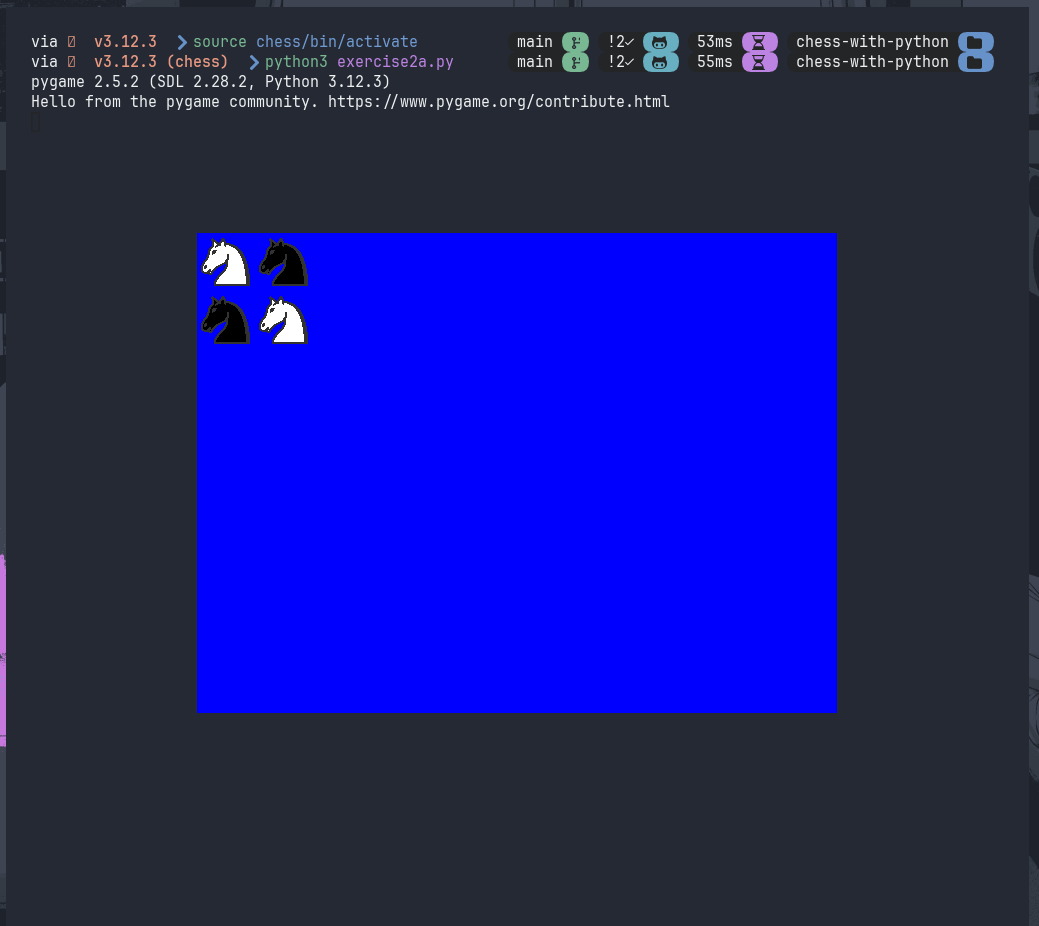
\includegraphics[width=0.8\textwidth]{img/exercise2a.png}
  \caption{Ejercicio 2A}
\end{figure}

\subsection{Ejercicio 2B}
Lo que nos pide es parecido al Ejercicio 2A, con la única deferencia que la referencia \mintpython{table} ahora la ponemos encima del mismo \mintpython{table} pero ya no invertido de color, sino con su espejo vertical. La acción de crear el espejo vertical de la figura \mintpython{table} la realizamos usando el método \mintpython{verticalMirror()}

\begin{minted}[bgcolor=background]{python}
from interpreter import draw
from chessPictures import *

table = knight.join(knight.negative())
table = table.up(table.verticalMirror())

draw(table)
\end{minted}

\begin{figure}[H]
  \centering
  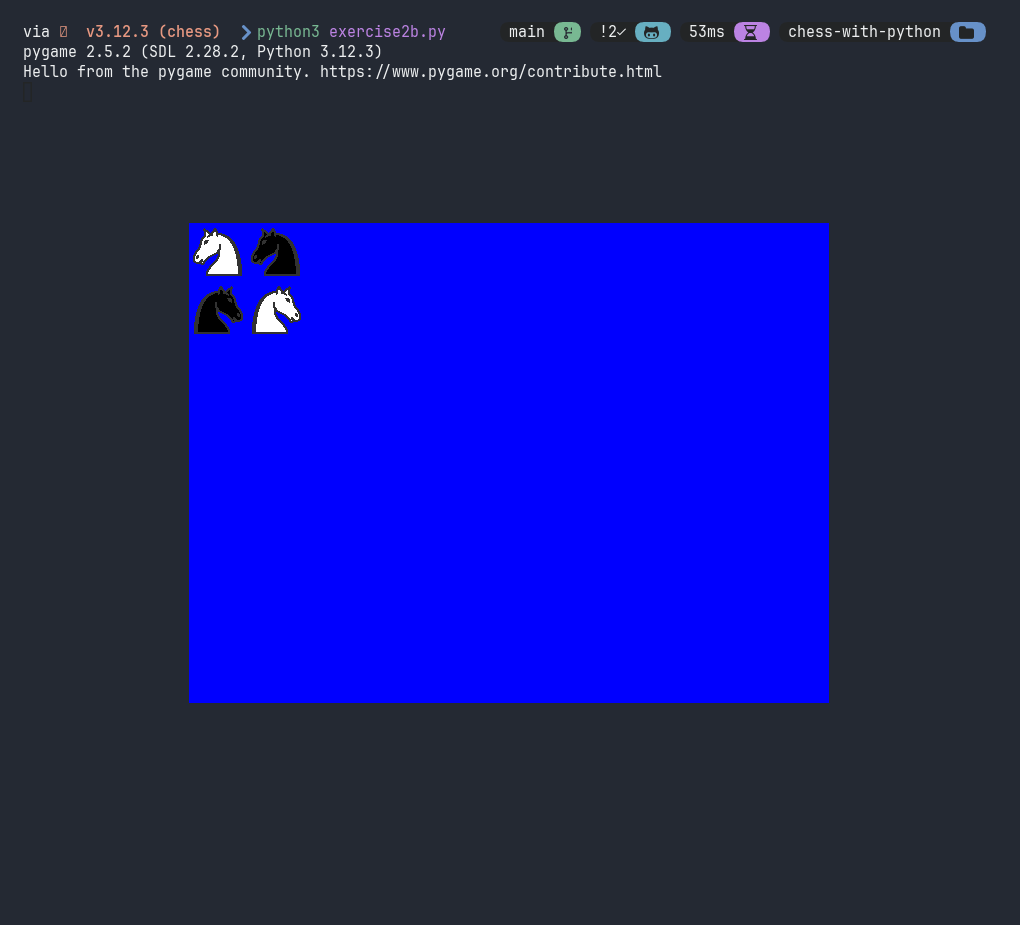
\includegraphics[width=0.8\textwidth]{img/exercise2b.png}
  \caption{Ejercicio 2B}
\end{figure}

\subsection{Ejercicio 2C}
El problema nos pide generar 4 reinas consecutivas a la derecha. El único método necesario que se usará es el método \mintpython{horizontalRepeat(n)} con el argumento de $ n = 4 $.

\begin{minted}[bgcolor=background]{python}
from interpreter import draw
from chessPictures import *

draw(queen.horizontalRepeat(4))
\end{minted}

\begin{figure}[H]
  \centering
  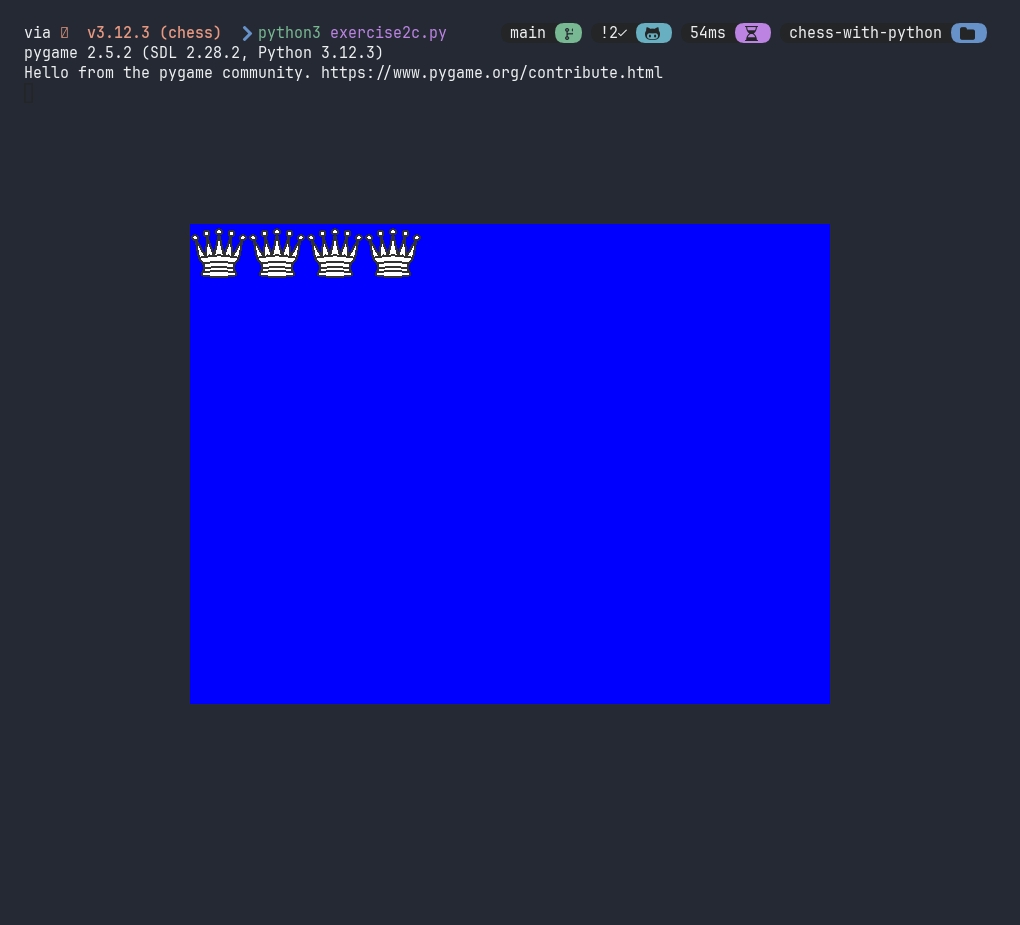
\includegraphics[width=0.8\textwidth]{img/exercise2c.png}
  \caption{Ejercicio 2C}
\end{figure}

\subsection{Ejercicio 2D}
Desde este problema en adelante nuestra lógica se basa en crear un patron base y manipularlo, cuando sea necesario, con todas los métodos que hemos implementado.
\singlespacing
El problema nos pide generar una fila de cuadrados intercalados de color, empezando con el cuadrado de color plomo o blanco. Rápidamente podemos imaginar que el patrón base es la figura \mintpython{square.join(square.negative())} y en este caso esta figura la repetimo 4 veces usando el método \mintpython{horizontalRepeat()}.

\begin{minted}[bgcolor=background]{python}
from interpreter import draw
from chessPictures import *

draw(square.join(square.negative()).horizontalRepeat(4))
\end{minted}

\begin{figure}[H]
  \centering
  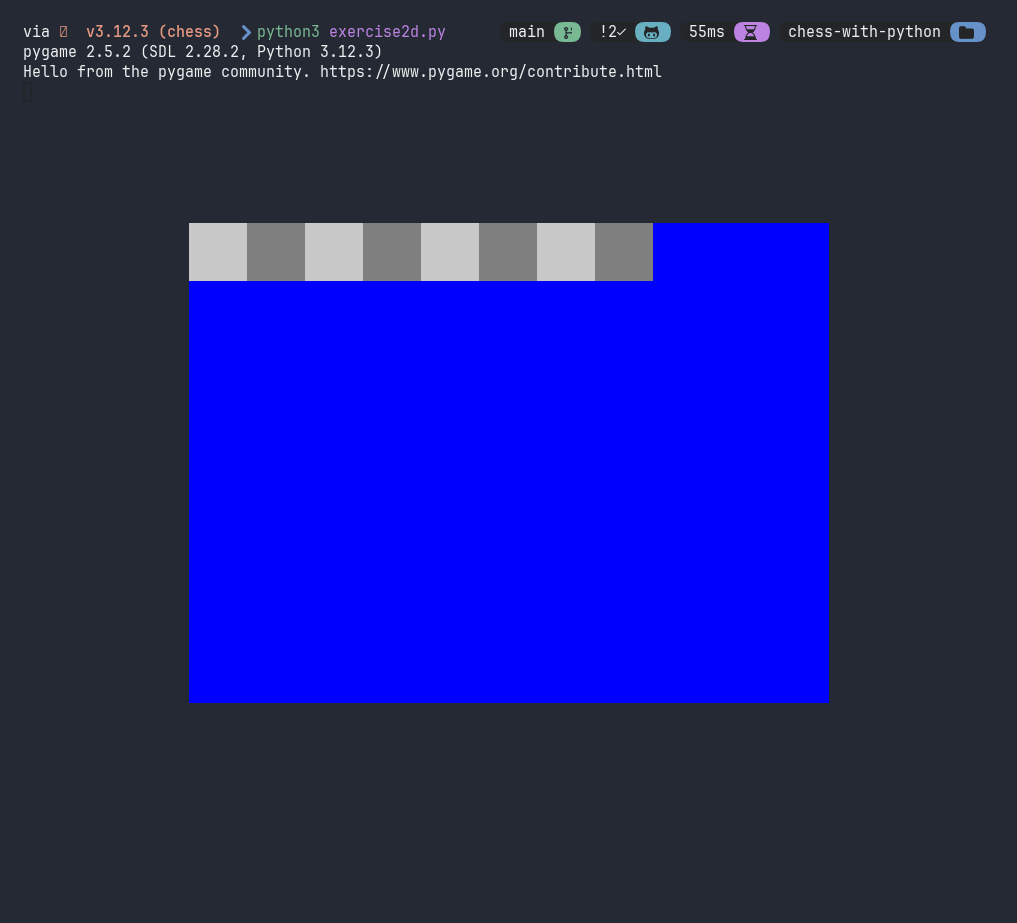
\includegraphics[width=0.8\textwidth]{img/exercise2d.png}
  \caption{Ejercicio 2D}
\end{figure}

\subsection{Ejercicio 2E}
Este problema nos pide lo mismo que el Ejercicio 2D pero empezando con el cuadrado de color negro. Entonces el patrón base ahora es la figura \mintpython{square.negative().join(square)} y esta la repetimos tambien 4 veces.

\begin{minted}[bgcolor=background]{python}
from interpreter import draw
from chessPictures import *

draw(square.negative().join(square).horizontalRepeat(4))
\end{minted}

\begin{figure}[H]
  \centering
  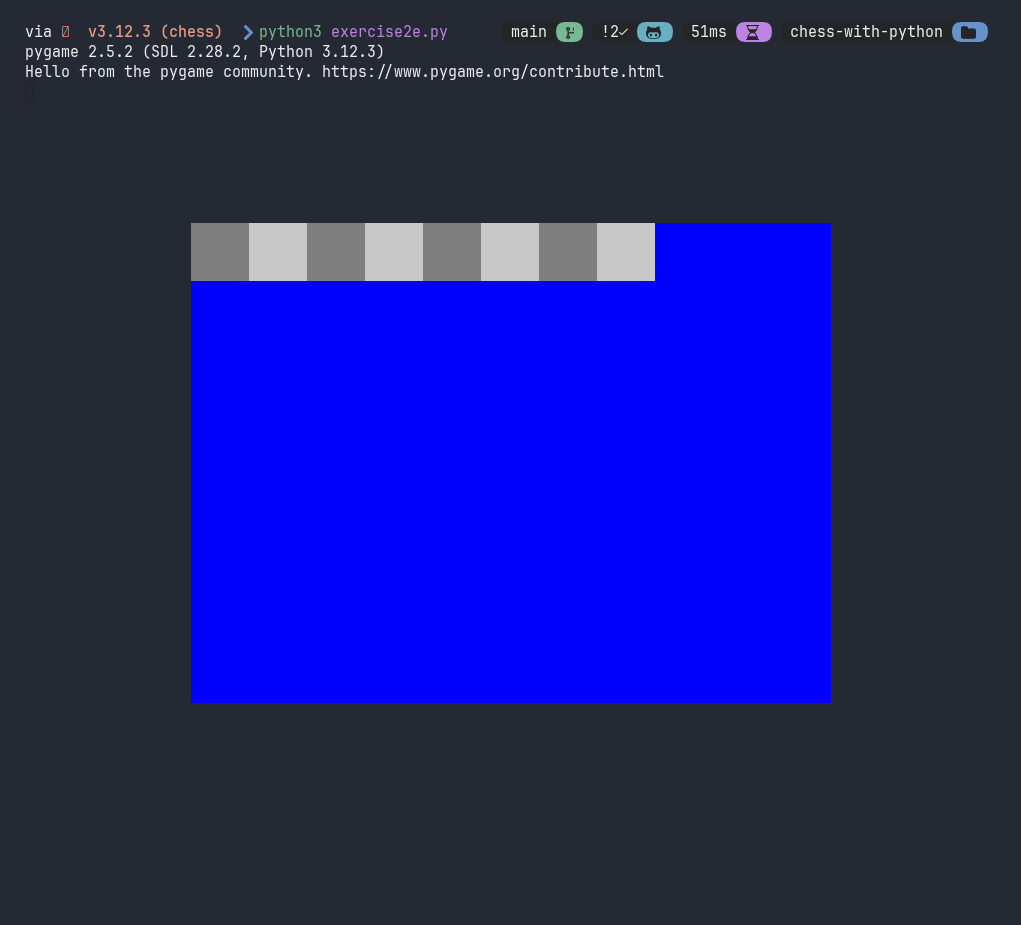
\includegraphics[width=0.8\textwidth]{img/exercise2e.png}
  \caption{Ejercicio 2E}
\end{figure}

\subsection{Ejercicio 2F}
El problema nos dice crear un tablero de ajedrez de 8x4 y empezando obviamente con el cuadrado blanco y asi intercalar los colores de los siguientes cuadrados. Entonces ahora podemos decir que nuestro patrón base será la primera fila del tablero, referenciaremos a este patrón con el nombre de \mintpython{table}. 
\singlespacing
Luego usamos este patrón para generar la segunda fila que simplemente es invertir los colores del patron o, tambien, es generar su espejo vertical. Hemos optado por usar \mintpython{negative()}.
\singlespacing
Finalmente hemos generado una figura de 2 filas con 8 columnas y solo nos queda repetirla verticalmente 2 veces. Para esta accion usamos el método \mintpython{verticalRepeat()}.

\begin{minted}[bgcolor=background]{python}
from interpreter import draw
from chessPictures import *

table = square.join(square.negative()).horizontalRepeat(4)
table = table.up(table.negative()).verticalRepeat(2)

draw(table)
\end{minted}

\begin{figure}[H]
  \centering
  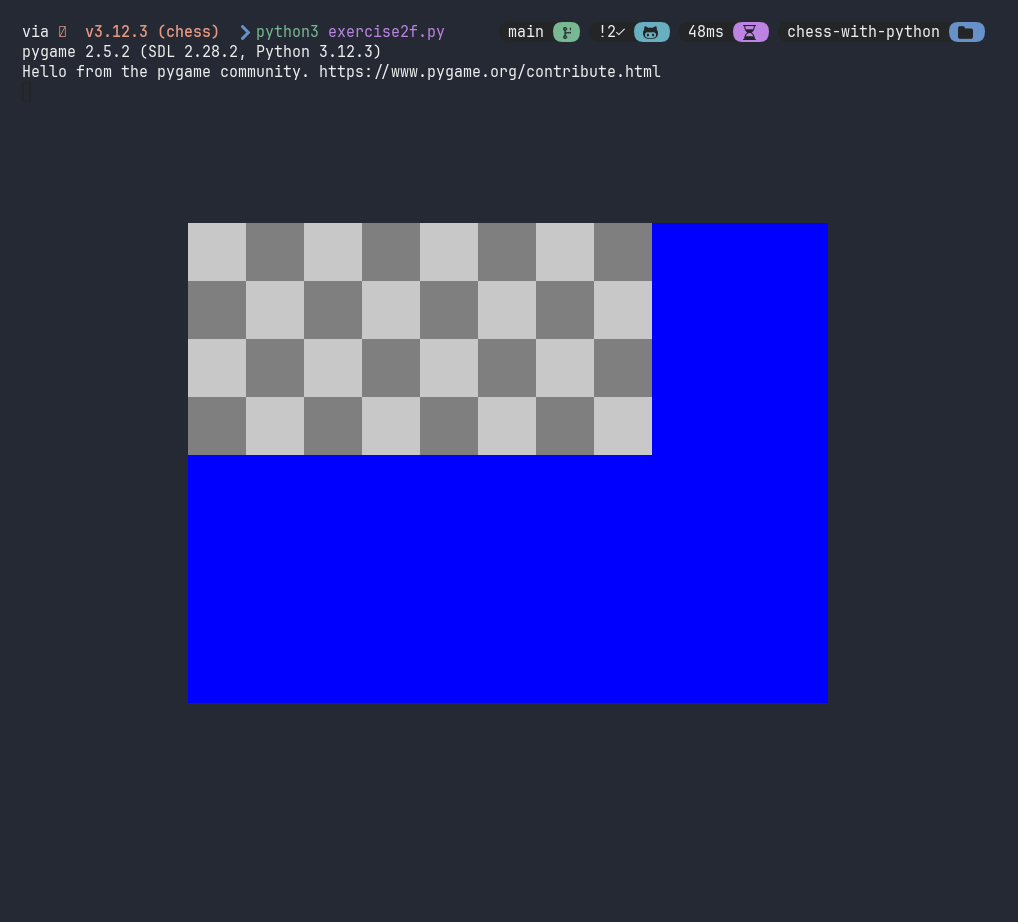
\includegraphics[width=0.8\textwidth]{img/exercise2f.png}
  \caption{Ejercicio 2F}
\end{figure}

\subsection{Ejercicio 2G}
Finalmente llegamos al problema donde nos pide crear un tablero de ajedrez completo con las fichas ordenadas. Se ha dividido en 3 partes que al final se deben de unir para conforma el tablero completo:

\begin{itemize}
  \item \textbf{Piezas negras:} Las piezas negras siempre van sobrepuestas sobre un tablero donde la pieza \textbf{torre} esta por encima del cuadrado blanco, y asi se intercalan los cuadrados. Esta parte la partimos en 2 partes más, pieces y paws:
    \begin{itemize}
      \item \textbf{Pieces:} Para generar la base de las piezas negras es la misma lógica que el Ejercicio 2D y esta figura la estamos referenciando con el identificador \mintpython{squares}. Ahora debemos generar la fila de las piezas, para ello hemos usado el método \mintpython{join()} colando uno a lado de otro todas las piezas y al final a toda esta fila de piezas la cambiamos de color con \mintpython{negative()}. Finalmente obreponemos la fila de piezas negras sobre \mintpython{squares} usando el método \mintpython{under()} y creando asi las Piezas negras.

      \item \textbf{Pawns:} Para crear las fila de peones, simplemente usamos el método \mintpython{horizontalRepeat()} y lo superponemos a \mintpython{squares}. Veremos aqui que tanto la fila de peones como la fila de \mintpython{squares} no coinciden con su color respectivo, por lo tanto a este resultado le cambiamos de color con \mintpython{negative()}. A
    \end{itemize} 
    Para culminar esta parte necesitamos colocar encima por encima de los peones negros, las piezas negras y esta acción la hacemos con \mintpython{up()}. A este resultado lo referenciamos con el identificador \mintpython{partBlack}

  \item \textbf{Tablero vacío:} Para esta parte simplemente usamos \mintpython{squares}, lo ponemos arriba de \mintpython{squares.negative()} y repetimos verticamente 2 veces. Esta figura la referenciamos como \mintpython{tableEmpty}.

  \item \textbf{Piezas blancas:} Para esta parte simplemente reutilizamos los resultados de \textbf{Piezas negras}. En vez de poner a los peones por debajo de las piezas como lo hicimos en esa sección, ahora lo hacemos al revez y al resultado le cambiamos de color con el método \mintpython{negative()}. Este resultado lo referenciamos con el identificador \mintpython{partWhite}
\end{itemize}

Finalmente tenemos que unir estas tres partes, colocando \textbf{Piezas negras} encima de \textbf{Tablero vacío} y este encima de \textbf{Piezas blancas}.

\begin{minted}[bgcolor=background]{python}
from interpreter import draw
from chessPictures import *

squares = square.join(square.negative()).horizontalRepeat(4)
piecesPart = rock.join(knight).join(bishop)

# Part black
pieces = squares.under(piecesPart.join(queen).join(king).join(piecesPart).negative())
pawns = squares.under(pawn.horizontalRepeat(8)).negative()
partBlack = pieces.up(pawns)

# Part empty
tableEmpty = squares.up(squares.negative()).verticalRepeat(2)

# Part white
partWhite = pawns.up(pieces).negative()

# table
table = partBlack.up(tableEmpty).up(partWhite)

draw(table)
\end{minted}

\begin{figure}[H]
  \centering
  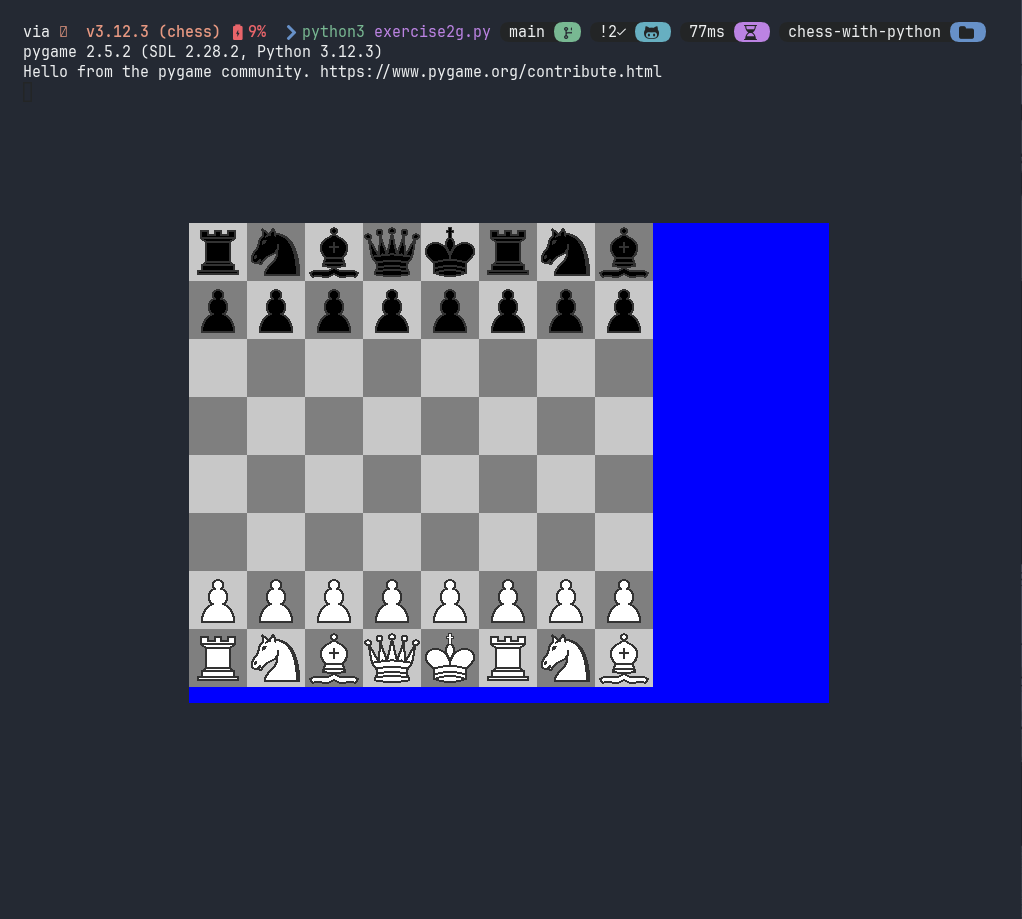
\includegraphics[width=0.8\textwidth]{img/exercise2g.png}
  \caption{Ejercicio 2G}
\end{figure}

\end{document}
